\section{Distributed File System}
A distributed file system enables programs to store and access remote files exactly as they do local ones, allowing users to access files from any computer on a network. The performance and reliability experienced for access to files stored at a server should be comparable to that for files stored on local disks. Distributed file systems support the sharing of information in the form of files and hardware resources in the form of persistent storage throughout a network.\\
Motivation for using distributed file system:
\begin{itemize}
	\item \textbf{availability}
	\item \textbf{fault tolerance}
	\item \textbf{performance} 
	\item \textbf{heterogeneity}
\end{itemize}

A distributed file system in general offers the following functionalities:
\begin{itemize}
	\item Sharing of resources
	\item Persistence for distributed shared objects.
	\item Distributed replicas of resources
	\item Consistency of resources, between multiple copies of data when updates occur. But respect to local file system it provides slightly weaker guarantees.
\end{itemize}

\subsection{File system modules}
The main role of a file system is to deal and manage files around the system. Each file contains data and a set of attributes used to make identify them or taking some decisions.
File systems are responsible for the organization, storage, retrieval, naming, sharing and
protection of files. They provide a programming interface that characterizes the file abstraction, freeing programmers from concern with the details of storage allocation and layout. Files contain both data and attributes. The \textbf{data} consist of a sequence of data items, accessible by operations to read and write any portion of the sequence. The \textbf{attributes} are held as a single record containing information such as the length of the file, timestamps, file type, owner’s identity and access control lists. The shaded attributes are managed by the file system and are not normally updated by user programs.\\
And it is organized in modules:

\begin{figure}[!h]
	\begin{minipage}[t]{0.5\linewidth}
		\centering
		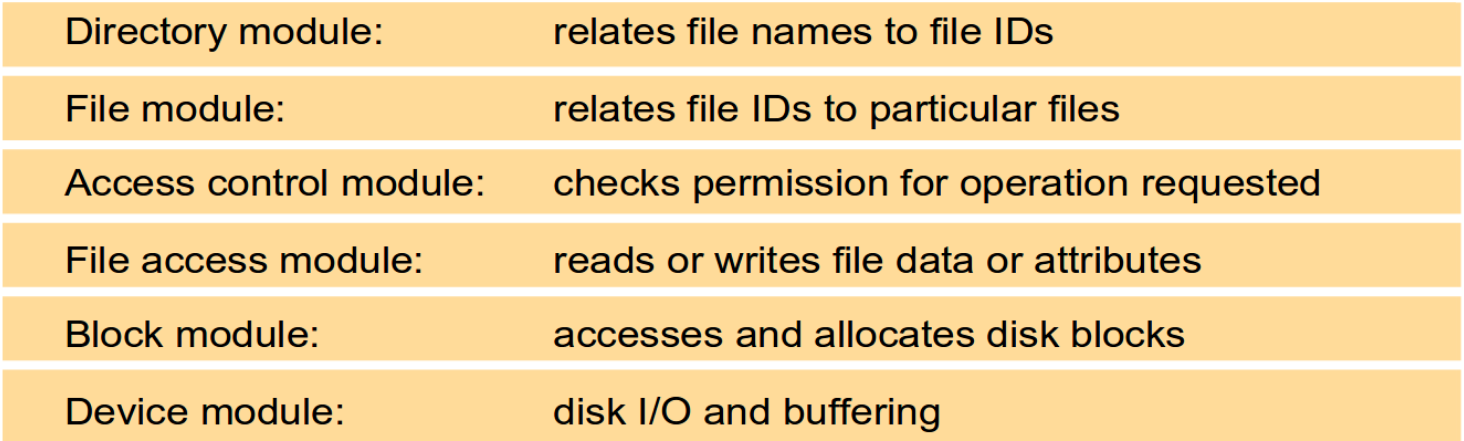
\includegraphics[width=1\textwidth]{img/fileSystemModules.png}
		\caption{File system modules}
		\label{f1}
	\end{minipage}
	\hspace{0.1cm}
	\begin{minipage}[t]{0.3\linewidth} 
		\centering
		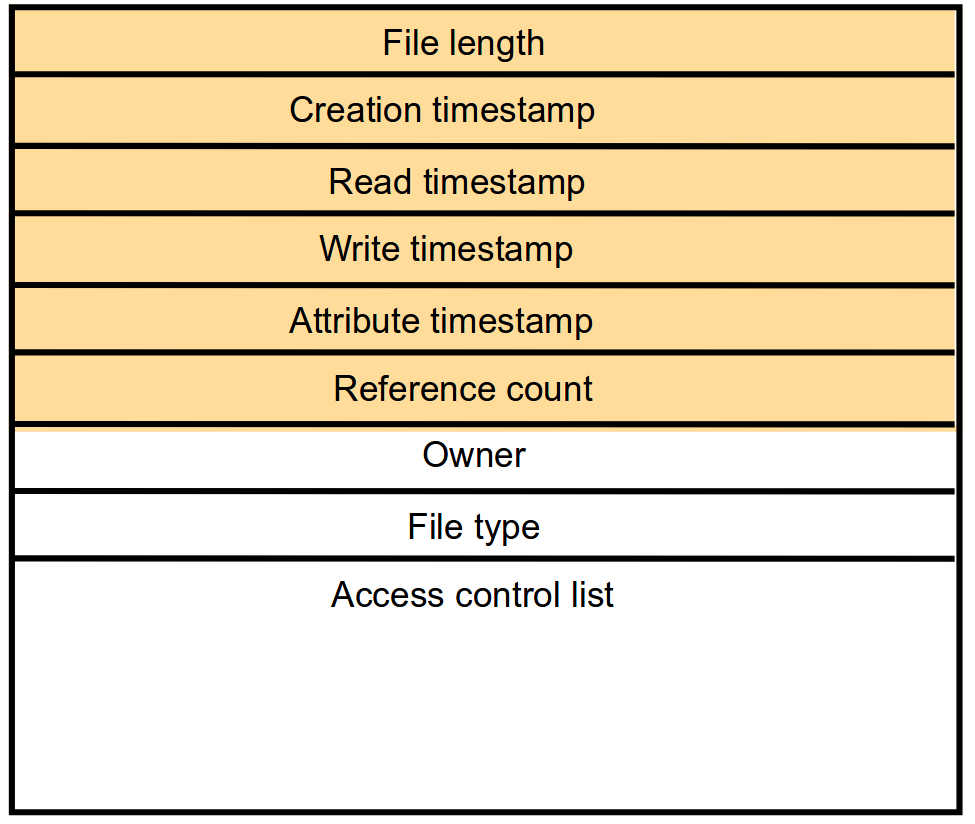
\includegraphics[width=1\textwidth]{img/fileAttributes.png}
		\caption{File attributes}
		\label{f2}
	\end{minipage}        
\end{figure}

\subsection{Distributed File System requirements}
In order to implement an useful distributed file system it is necessary to consider the following requirements:
\begin{itemize}
	\item \textbf{Transparency}, the design must balance the flexibility and scalability that derive from transparency against software complexity and performance. The following forms of transparency are provided:
	\begin{itemize}
		\item \textit{Access transparency}, clients does not have knowledge on how to resources are accessed by the system.
		\item \textit{Location transparency}, clients are not affected by possible change of locations of resources.
		\item \textit{Performance transparency}, clients see always the same level of performance.
		\item \textit{Scalability transparency}, the service can be expanded by incremental growth to deal with a wide range of loads and network sizes.
		\item \textit{Mobility transparency}, if files are moved clients are not affected.
	\end{itemize}
	    
	
	\item \textbf{Concurrency}, changes to a file by one client should not interfere with the operation of other clients simultaneously accessing or changing the same file.
	
	\item \textbf{Replication}, in a file service that supports replication, a file may be represented by several copies of its contents at different locations. This has two benefits – it enables multiple servers to share the load of providing a service to clients accessing the same set of files, enhancing the scalability of the service, and it enhances fault tolerance by enabling clients to locate another server that holds a copy of the file when one has failed.
	
	\item \textbf{Heterogeneity}, The service interfaces should be defined so that client and server software can be implemented for different operating systems and computers.
	
	\item \textbf{Consistency}, when files are replicated or cached at different sites, there is an inevitable delay in the propagation of modifications made at one site to all of the other sites that hold copies, and this may result in some deviation from one-copy semantics.
	
	\item \textbf{Fault Tolerance}, the central role of the file service in distributed systems makes it essential that the service continues to operate in face of client and server failures.
	
	\item \textbf{Security}, there is a need to authenticate client requests so that access control at the server is based on correct user identities and	to protect the contents of request and reply messages with digital signatures and encryption of secret data.
	
	\item \textbf{Efficiency}, a distributed file service should offer facilities that are of at least the same power and generality as those found in conventional file systems and should achieve a comparable level of performance.
\end{itemize}

\subsection{Case of study}
In this section we are going to study some particular file systems implementation.

\subsubsection{File service architecture}
The architecture is designed to enable a stateless implementation of the server module. It structures the file service as three components \textbf{flat file service}, a \textbf{directory service} and a \textbf{client module}.

\image{img/fileService.png}{File Service Architecture}{0.6}

The \textbf{flat file service} is concerned with implementing operations on the contents of files. \textit{Unique file identifiers} are used to refer to files in all requests for flat file service operations. The implemented operations are idempotent.\\
The \textbf{directory service} provides a mapping between text names for files and their UFIDs. The directory service provides the functions needed to generate directories, to add new file names to directories and to obtain UFIDs from directories.\\
The \textbf{client module} also holds information about the network locations of the flat file server and directory server processes.

\subsubsection{Sun Network File System}
\textbf{Sun Network File System} is implemented though \textbf{NFS protocol}, which is a set of remote procedure calls that provide the means for clients for perform operations on a remote file store. NFS provides access transparency, user programs can issue file operations for local or remote files without distinction. It is composed by NFS Server and NFS Client, that communicate using remote procedure calls.\\
The \textbf{NFS Server module} is stored in the kernel on each computer that acts as an NFS server. Requests referring to files in a remote file system are translated by the client module to NFS protocol operations and then passed to the NFS server module at the computer holding the relevant file system.
The \textbf{NFS client module} cooperates with the virtual file system in each client machine. It operates in a similar manner to the conventional UNIX file system, transferring blocks of files to and from the server and caching the blocks in the local memory whenever possible.\\
\image{img/NFSarchitecture.png}{Sun Network File System}{0.7}

To use a remote file system the process uses \verb|mount service| available on every server NFS. Each server has to sign the list of the exportable file systems, and each client can mount them using \verb|mount| command specifing server name and the paths.

Caching in both the client and the server computer are indispensable features of NFS implementations in order to achieve adequate performance

The server keeps in local memory blocks of files belonging to the exported file system. It is necessary to deal with consistency of data, and for that reason two strategies are adopted:
\begin{itemize}
	\item \textbf{Write Through}, block are written on the disk when the server receives the write request by a client.
	\item \textbf{Write back}, blocks are not immediately written on the disk at the receiving time of the write request. Client can invoke the primitive \verb|commit| to ask to the server to write all the blocks in the cache.
\end{itemize}
The client module caches the results of read and write operations, reducing the request number to the server. The main problem is that there can be different versions of the same file in different nodes, and so the solution is to assign the client the responsibility to check for data consistency in its cache. For every access to a shared file one has to verify the \textbf{validity cache condition}. Each element in the cache of the client has $T_c$, time of last validation, $T_m$, time of last modification. Chosen a threshold $t$ it is necessary to verify that the time from last validation must not be greater than $t$.


\subsubsection{Andrew File System}
Like NFS allows the applications to access remote file systems without recompilation. AFS with respect to NFS has more \textbf{scalability} and it allows the following main features:
\begin{itemize}
	\item Files are entirely transferred by the server to the clients in one operation.
	\item Clients keep in their own a cache local copy of the file (entire) received by the server.
\end{itemize}
AFS is designed to perform well with larger numbers of active users than other distributed file systems. The key strategy for achieving scalability is the caching of whole files in client nodes.\\

AFS is implemented as two software components that exist as UNIX processes called \textbf{Vice} and \textbf{Venus}.

\image{img/AndrewArchitecture.png}{Andrew file system architecture}{0.6}
Venus is a client working at upper level in each workstation, and Vice is a server that works at upper level. In other words: Vice is the name given to the server software that runs as a user-level UNIX process in each server computer, and Venus is a user-level process that runs in each client computer and corresponds to the client module in our abstract model. The file system of each workstation is formed by local files, not shared, and shared files, stored on the server and copies are cached on the local disks of workstations.\\
When a process in a workstation client open a remote file, and if there is no copy in the local cache the file is localized and a copy is required. That copy is stored in the local file system.
Successive read/write operations of the process work on the local copy.\\
When the process close the file: if the local copy has been modified  then it is sent back to the server, otherwise the copy is kept in the workstation for possible successive requests. In general read and write operations are not so frequent and the local cache is very large.\\
Andrew file system assumes:
\begin{itemize}
	\item most of the file are small
	\item read is more frequent than write
	\item sequential access is more common
	\item most of the file are modified only by one client 
	\item file are often used as burst.
\end{itemize}
So it could be not reasonable to use Andrew file system for database.\\
One of the most important problem is given by \textbf{Consistency of the cache}. When a module Vice (server) gives a file to Venus (client) it also sends a \textbf{callback promise}, which is a promise of the server to contact later the client when the file is modified by other clients. In the client cache to each file there is the callback associated and it can be in two possible states: \textbf{valid}, the server has not yet communicated the file changes, \textbf{cancelled}, the server did a recall communicating to invalidate the local copy of the file because of changes.
When a server receives the change request of a file, it send a message to all those clients to which it previously promised a \textbf{callback}. Once connected by the server, the client put the callback associated to that file as cancelled. AFS is not stateless respect to NFS. \\

Another aspect that should be considered is the \textit{fault tolerance}. When a workstation starts again after crash it must try to keep most of the content of its cache. It could have lost some callback by the server and so the cache has to be validated again. \textbf{Revalidation} of the cache works as follow:
\begin{itemize}
	\item the client sends a cache validation request with the file to be validated and the date of the last change.
	\item if the server verifies that there were no changes starting from the date indicated by the client, then the file and the corresponding callback is validated. 
	\item Otherwise the callback is set as cancelled. 
\end{itemize}
In any case, each client has to validate again a callback once some time elapsed without receiving any server notification. Note also that this consistency strategy is applied only during \verb|open| or \verb|close| operations, and it is possible that different clients try to change at the same file so producing incosistent results.